\documentclass[12pt,a4paper]{article}
\usepackage[spanish]{babel}
\usepackage[utf8]{inputenc}
\usepackage[T1]{fontenc}
\usepackage{geometry}
\usepackage{graphicx}
\usepackage{hyperref}
\usepackage{float}
\geometry{margin=2.5cm}

\title{Bitacora del Taller - Lenguajes de Programacion}
\author{Antonio}
\date{\today}

\begin{document}
\maketitle

\section{Punto 1 y 2}
\subsection*{Objetivo}
Implementar un mini lenguaje CRUD con ANTLR en Python y un visitante de evaluacion en memoria.

\subsection*{Lo realizado}
\begin{itemize}
    \item Se definio la gramatica en \texttt{punto\_1\_\&\&\_2/gramatica/LenguajeNoRelacional.g4}.
    \item Se implemento el analizador en \texttt{punto\_1\_\&\&\_2/analizador.py}.
    \item Se implemento la evaluacion con visitante en \texttt{punto\_1\_\&\&\_2/visitante\_evaluacion.py}.
    \item Se incluyo ejemplo de ejecucion y prueba automatizada.
\end{itemize}

\subsection*{Evidencia (espacio para imagen)}
\begin{figure}[H]
    \centering
    \fbox{\rule{0pt}{6cm}\rule{0.9\linewidth}{0pt}}
    \caption{Captura de ejecucion del punto 1 y 2 (agregar imagen).}
\end{figure}

\section{Punto 3}
\subsection*{Objetivo}
Calcular PRIMEROS, SIGUIENTES y PREDICCION para verificar propiedades relacionadas con LL(1).

\subsection*{Lo realizado}
\begin{itemize}
    \item Se trabajo con los scripts de \texttt{punto\_3} para procesar gramaticas desde archivo.
    \item Se ejecuto \texttt{python ASD\_Recursivo.py gramatica1.txt} para obtener tablas de salida.
    \item Se uso como referencia de apoyo el repositorio previo de la materia y la explicacion teorica de LL(1):
    \begin{itemize}
        \item \url{https://www.quora.com/How-can-you-prove-or-explain-with-words-that-an-LL-1-grammar-only-needs-one-lookahead-if-you-make-a-recursive-descent-parser-form-it}
    \end{itemize}
\end{itemize}

\subsection*{Evidencia del punto 3}
\begin{figure}[H]
    \centering
    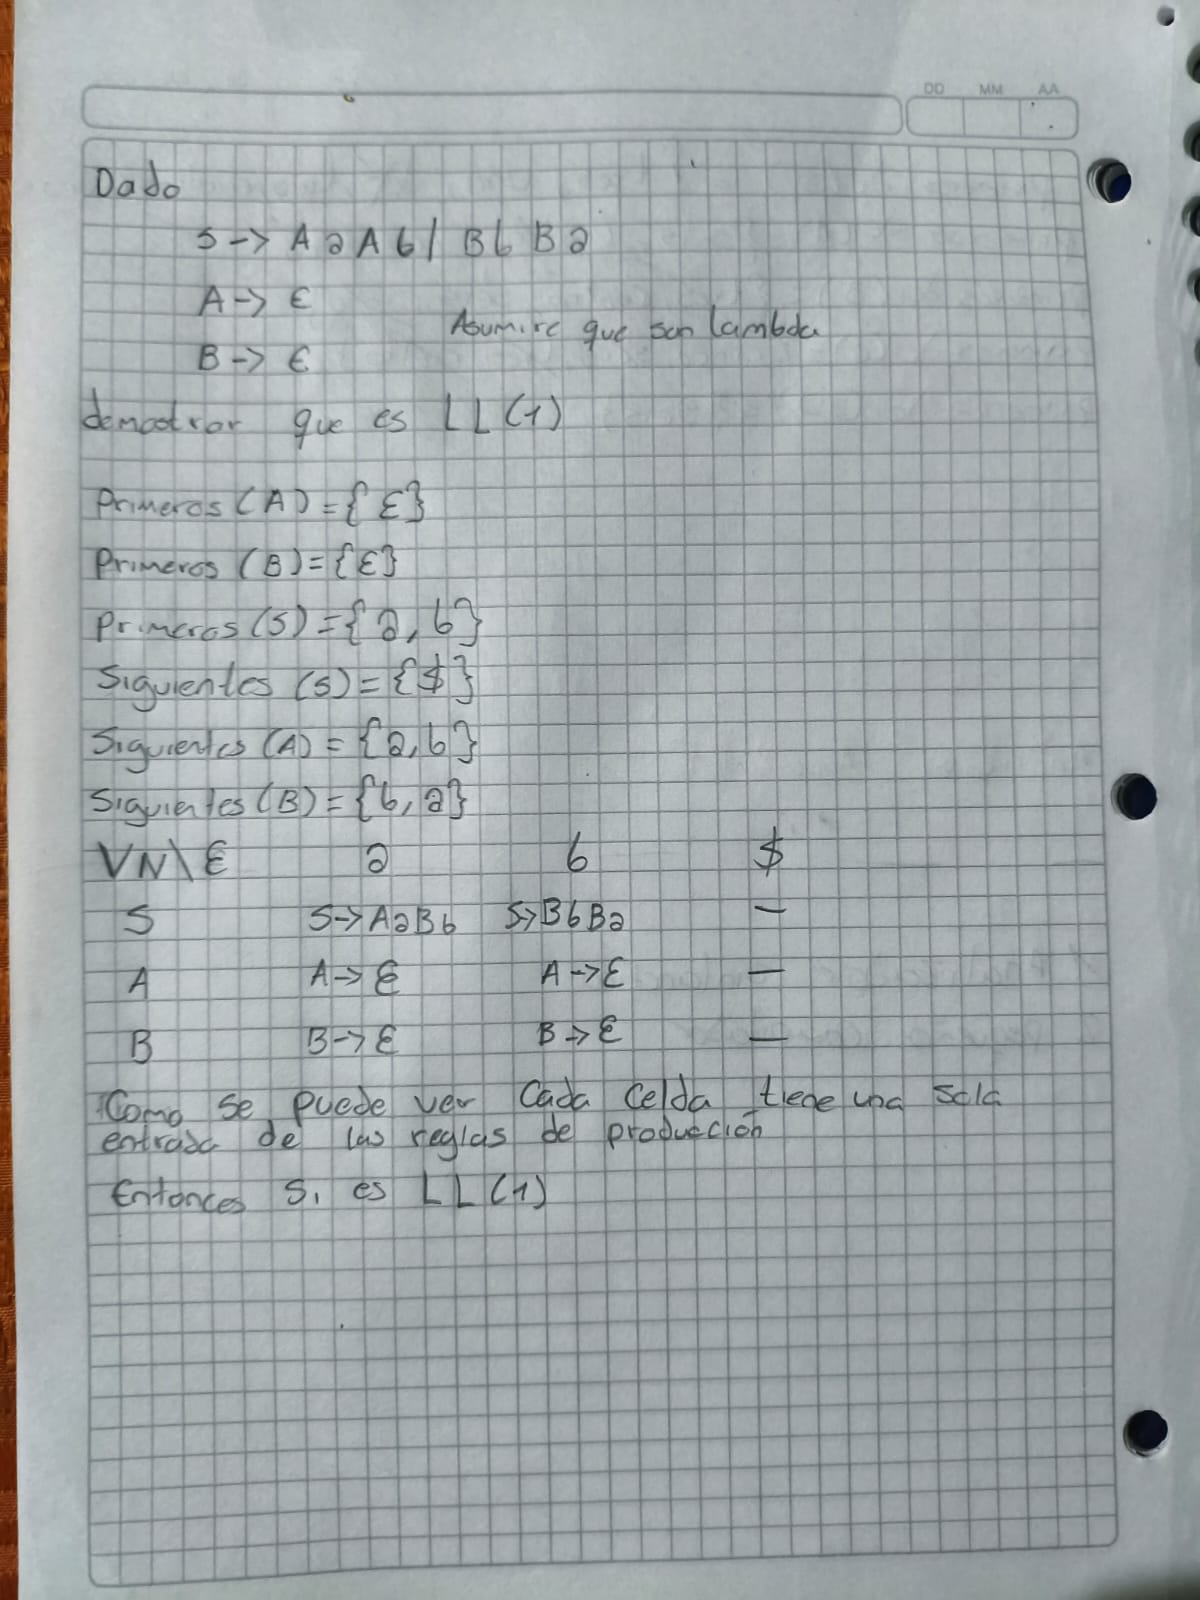
\includegraphics[width=0.85\linewidth]{punto_3/Prueba.jpeg}
    \caption{Evidencia de ejecucion del punto 3.}
\end{figure}

\subsection*{Espacio adicional para otra imagen}
\begin{figure}[H]
    \centering
    \fbox{\rule{0pt}{6cm}\rule{0.9\linewidth}{0pt}}
    \caption{Imagen adicional del punto 3 (opcional).}
\end{figure}

\end{document}
